\documentclass{article}
\usepackage{graphicx} % new way of doing eps files
\usepackage{listings} % nice code layout
\usepackage[usenames]{color} % color
\usepackage{float}
\definecolor{listinggray}{gray}{0.9}
\definecolor{graphgray}{gray}{0.7}
\definecolor{ans}{rgb}{1,0,0}
\definecolor{blue}{rgb}{0,0,1}
% \Verilog{title}{label}{file}
\newcommand{\Verilog}[3]{
  \lstset{language=Verilog}
  \lstset{backgroundcolor=\color{listinggray},rulecolor=\color{blue}}
  \lstset{linewidth=\textwidth}
  \lstset{commentstyle=\textit, stringstyle=\upshape,showspaces=false}
  \lstset{frame=tb}
  \lstinputlisting[caption={#1},label={#2}]{#3}
}


\author{Justin Roessler and Jon Johnston}
\title{Lab 3 Fetch Stage}

\begin{document}
\maketitle

\section{Executive Summary}
The purpose of this lab is to finish the fetch stage of our arm processor. The fetch stage updates the PC with each positive clock edge(add 4), reads the value of the program counter, takes the information at that memory location, and sends it out to the next stage to be executed. The fetch stage can also jump to a branch address if the pc\_src is set to 1. 

A mux was used to switch between the program counter's address and the branch address depending on the pc\_src. Also, an add module was used to add 4 to the PC with each positive clock edge. Lastly, an instruction memory module was created to take the address location from the mux and output the contents of that address to the decode stage of the processor. After implementing some delays and these modules, the lab was a success and the fetch stage is operating as expected.


\section{Test Report}
To verify operation of this/these module(s), this lab requires 2 test benches. 
\begin{enumerate}
	\item Instruction Memory Test Bench
	\item Fetch Test Bench
\end{enumerate}

% This section should display the Expected Results Table and the Simulation Results for each test bench.  Make sure to label each figure correctly.  Please put them in the order of ERT1, SimResults1, ERT2, SimResults2 so that I can easily compare the ERT and Simulation Results.  To force the figures to be positioned correctly, add the float package (at the top of this file) and use the [H] after {figure} as I did below.  Also, if the ERT is on one page and the Simulation Results are on the next page, you can use a pagebreak as I did below so that the ERT goes to the next page also.

\pagebreak

\begin{figure}[H]
	\begin{center}
		\caption{Expected Results of the Instruction Memory test.}\label{fig:ert_instmemtest}
		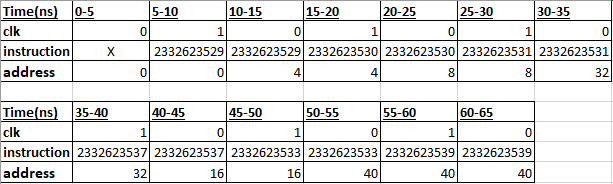
\includegraphics[width=1.0\textwidth]{../images/InstrMemExpected.png}
	\end{center}
\end{figure}

\begin{figure}[H]
	\begin{center}
		\caption{Timing Diagram for the Instruction Memory test.}\label{fig:instmemtest}
		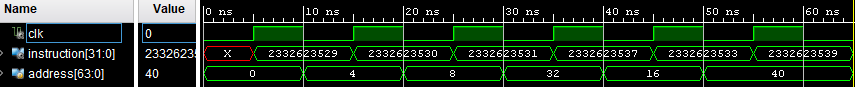
\includegraphics[width=1.0\textwidth]{../images/InstrMemSimulation.png}
	\end{center}
\end{figure}

\begin{figure}[H]
	\begin{center}
		\caption{Expected Results of the Fetch test.}\label{fig:ert_fetchtest}
		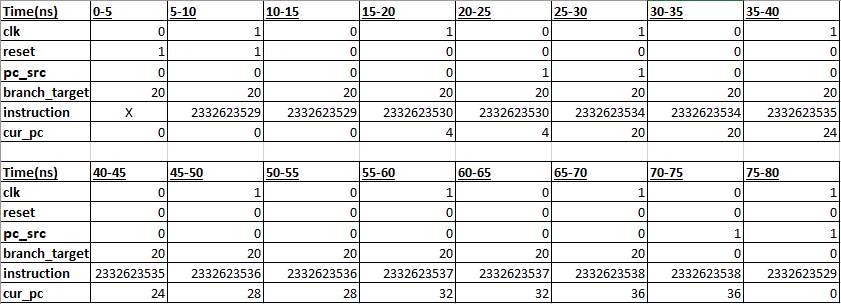
\includegraphics[width=1.0\textwidth]{../images/FetchExpected.png}
	\end{center}
\end{figure}

\begin{figure}[H]
	\begin{center}
		\caption{Timing diagram for the Fetch test.}\label{fig:fetchtest}
		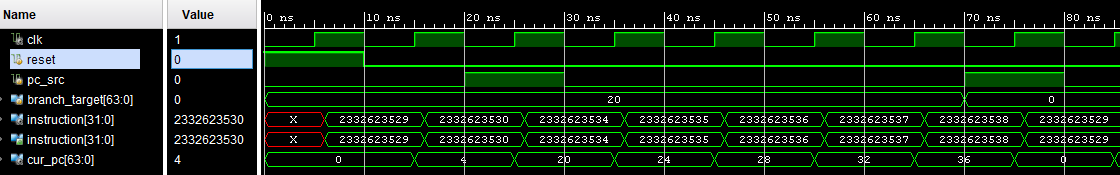
\includegraphics[width=1.0\textwidth]{../images/FetchSimulation.png}
	\end{center}
\end{figure}

\pagebreak
\section{Code Appendix}
% The code appendix should include the test bench code and module code for this lab.
\Verilog{Verilog code for testing a Instruction Memory.}{code:regtest}{../code/1_fetch/instr_mem_test.v}
\Verilog{Verilog code for implementing a Instruction Memory.}{code:reg}{../code/1_fetch/instr_mem.v}
\Verilog{Verilog code for testing the Fetch Stage.}{code:reg}{../code/1_fetch/fetch_test.v}
\Verilog{Verilog code for implementing the Fetch Stage.}{code:reg}{../code/1_fetch/fetch.v}
\end{document} 